\begin{figure*}[htb!]
\centering
\includegraphics[width=\textwidth]{images/volumetric/results}
\caption[Volumetric NED: results]{View through our volumetric near-eye display where virtual objects are placed among real objects at a range of distances. \emph{Extreme left:} Overhead depiction of scene geometry. Icons to the left of the optical axis correspond to virtual objects, while icons to the right of the optical axis correspond to real objects. \emph{Other images, left to right, in each row:} Photos taken through the display where the focus of the camera is adjusted progressively from near to far. In each row, the only difference between the see-through views is the camera's focus settings - this demonstrates the ability of the display to provide proper focus cues for all virtual pixels simultaneously, allowing the viewer to freely accommodate in the scene without any feedback to the display.}
\label{fig:volumetric:results}
\end{figure*}


\subsection{Results}
\label{sec:volumetric:results}
\paragraph{Cameras}
To record images and videos of the see-through view of the display, cameras that approximate the human eye were placed behind the display (see Figure~\ref{fig:volumetric:setup}) at a distance that approximated the eye relief of a human viewer (2cm away from the beamsplitter). See-through image results presented in this chapter were recorded using a Canon T6i Rebel camera with a Canon 24-70mm f/2.8 lens. See-through video results (in accompanying video submission) were recorded using a Point Grey Chameleon3 camera with a Fujinon 2.8-8mm f/1.2 lens. A 4mm aperture was used in both cameras to emulate the human pupil diameter while collecting results. When using PointGrey cameras, the nearest distance was chosen to be 15cm (6.7 diopters), and when using the DSLR camera, the minimum distance was 20cm (5 diopters) because the lens could not focus closer. 

Our display is capable of presenting virtual imagery closer than 15cm and farther than 4M, but we were constrained by the recording camera (for the minimum distance) and by the lab space (for the farthest distance). Although virtual images closer or farther than what is demonstrated here may not be required for near-eye displays, this may be of use in some other application.

\paragraph{Setup}
Figure~\ref{fig:volumetric:setup} shows the monocular display prototype, the positioning of the camera in place of a viewer's eye and the staged real-world scene consisting of a large poster, and smaller objects such as a Rubik's cube, a wristwatch and a tiny rubber ducky (2cm height). The real-world objects are arranged from small to large progressively away from the display approximately along the line of sight of the see-through view. Virtual objects are scaled progressively from small to large away from the display for the virtual objects to subtend approximately the same angle at the camera. 

\paragraph{See-through images}
Figure~\ref{fig:volumetric:results} shows the see-through views of our NED when displaying a virtual scene registered to the staged real-world scene. Even though our RGB LED illuminator can produce high-dynamic range and consequentially very bright virtual imagery~\cite{Lincoln2017scene}, we're currently displaying moderately bright imagery at 24 bits-per-pixel. A black background screen is used to improve the visibility and contrast of the virtual objects.

As discussed earlier, the field of view of the virtual image changes during the lens cycle. Ideally, this needs to be calibrated for, but we didn't. Other first-order and second-order optical aberrations present in all optical systems may also need to be calibrated. Each of these optical aberrations likely varies with depth across the volume. Optical aberrations are observable in our system, e.g., in the second row of Figure~\ref{fig:volumetric:results}, even when focused at the correct depth, the bottom portion of the Jack card is blurred relative to the top. 

To demonstrate that our display shows high-resolution imagery when each binary image is considered individually, Figure~\ref{fig:volumetric:single_plane_images} shows the see-through view when only one of the 280 binary images was encoded with the image of a wire model of a teapot. 

\begin{figure}[htb!]
\centering
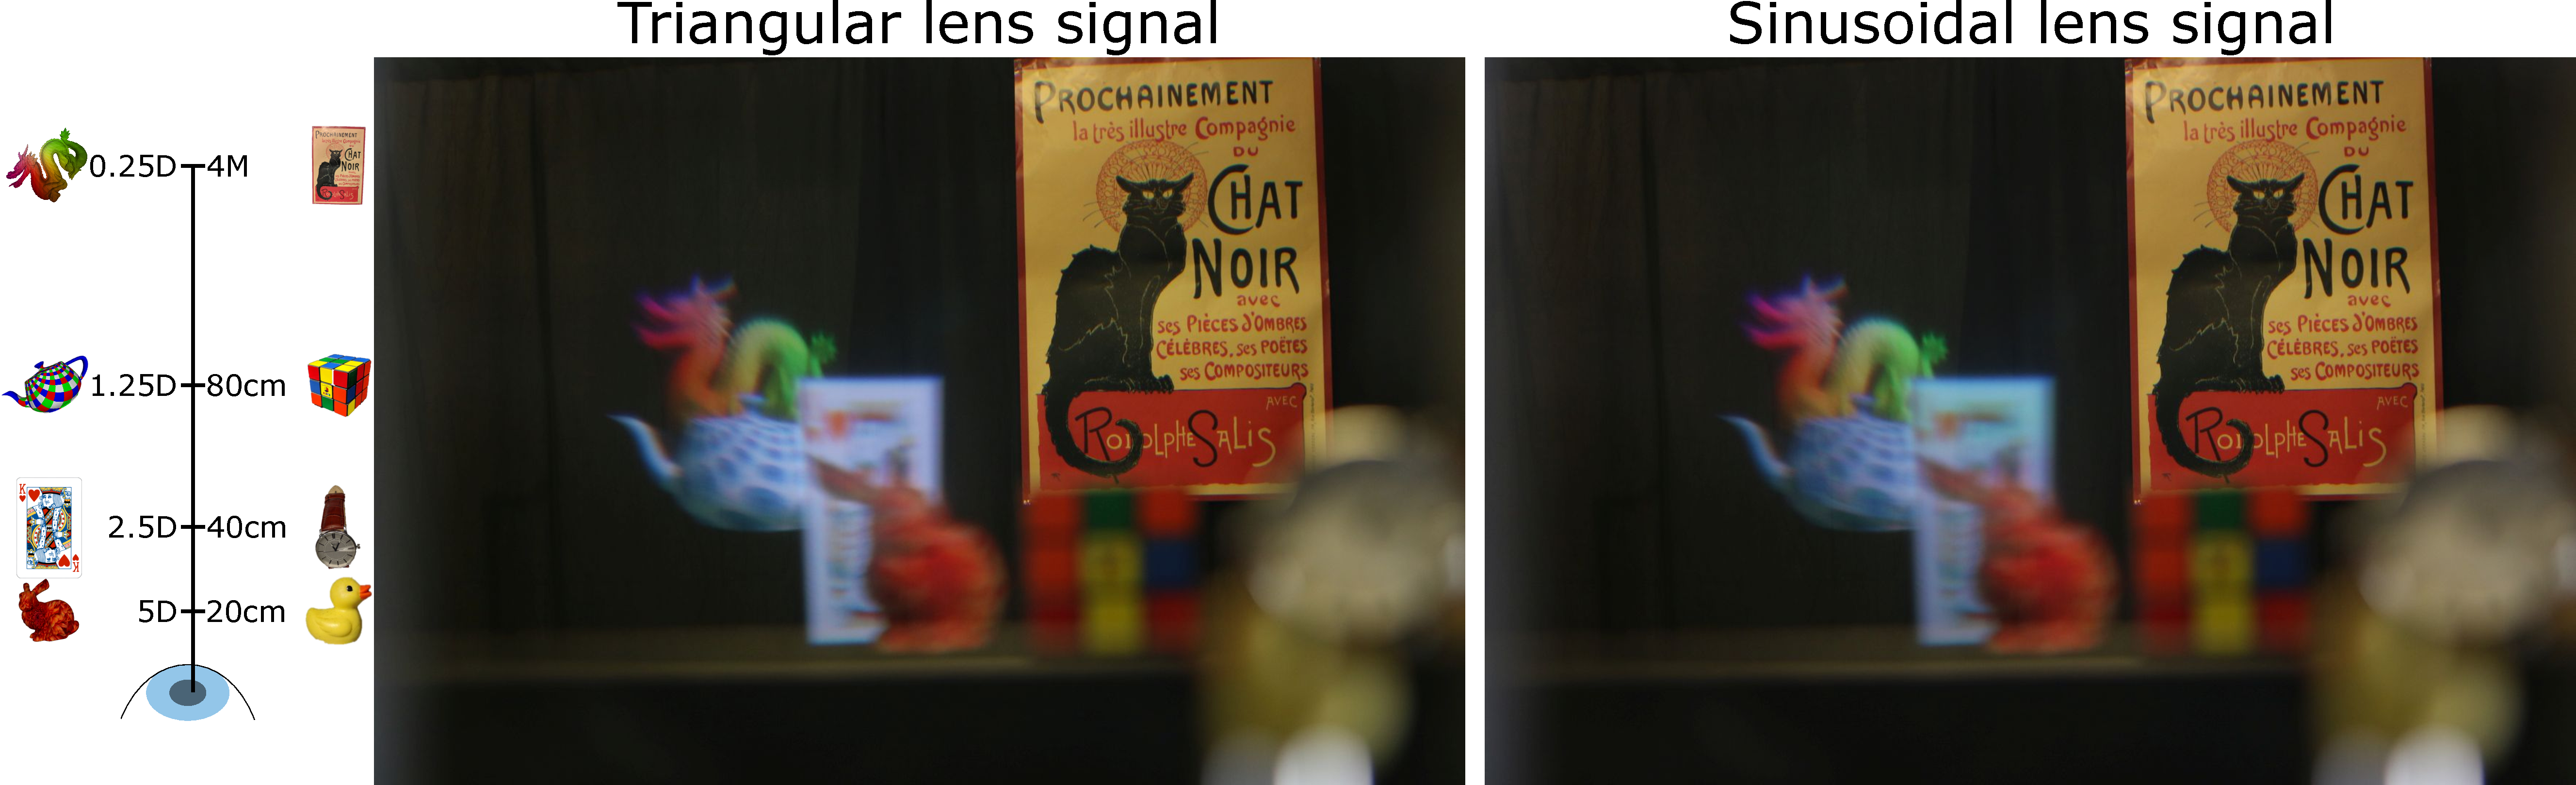
\includegraphics[width=\columnwidth]{images/volumetric/sinusoidal_vs_triangular}
\caption[Volumetric NED: Sinusoidal vs. triangular lens functions]{Images show the see-through view through the display when the optical power of the focus-tunable lens follows a triangular waveform and a sinusoidal waveform. For both these images, the voxelization and color volume to binary volume decomposition was performed assuming a triangular waveform. We don't observe a significant difference in the see-through images.}
\label{fig:volumetric:sinusoidal_vs_triangular}
\end{figure}


Figure~\ref{fig:volumetric:sinusoidal_vs_triangular} shows a comparison between the see-through views when the lens signal follows a triangular and a sinusoidal waveform. This is discussed in Section~\ref{sec:volumetric:sinusoidal_vs_triangular}.


\paragraph{Video results}
A video was recorded as a demonstration of this display. This video was submitted as part of this dissertation and is also available publically at this URL: \url{https://www.youtube.com/watch?v=oDcOQ_NotRU}. 
The video results show a larger range of depth (15cm - 4M) compared to the image results (20cm - 4M) because the camera used to record the video was able to focus closer. In these videos, a flicker is seen propagating back and forth through the displayed volume. This flicker is an artifact of the video capture and is not human-visible. The flicker arises because of the slight discrepancy between the display frame time (16.67 ms) and the minimum shutter speed possible on the camera (16.74 ms). The flicker moves back and forth in the volume because the camera samples the whole volume once and a small portion of the volume twice - and because of this, it starts to sample the volume in the subsequent frame from a slightly different starting position of the volume. 

